% ===============================================================
%  جلسه سیزدهم
% ===============================================================
\chapter{توزیع مشترک دو یا چند متغیر تصادفی}

\section{توزیع مشترک دو متغیر تصادفی \lr{(Joint Distributions)}}

\subsection{انگیزه}
دو متغیر تصادفی $X$ و $Y$ با توزیع‌های انباشته $F_X$ و $F_Y$ را در نظر بگیرید:
\[
F_X(x)=\Prob(X\le x),\qquad F_Y(y)=\Prob(Y\le y).
\]
در صورتی که در مورد استقلال این دو متغیر تصادفی هیچ فرضی نکنیم، در مورد احتمال وقایعی مانند زیر چه حرفی می‌توان زد؟
\[
\Prob(0\le X\le2\ ,\ Y>3)
\]
\begin{itemize}
\item \textbf{در صورت برقرار استقلال آماری میان $X,Y$}، می‌توان احتمال کل را به صورت ضرب احتمال وقایع نوشت:
$\Prob(0\le X\le2)\Prob(Y>3)=\big(F_X(2)-F_X(0^-)\big)\big(1-F_Y(3)\big)$.
\item \textbf{در صورت نبود هیچ فرضی در مورد استقلال دو متغیر تصادفی}، به اطلاعاتی فراتر از توزیع جداگانه آنان نیاز خواهیم داشت. توزیع‌های حاشیه‌ای (جداگانه) فقط رفتار هر متغیر را به تنهایی توصیف می‌کنند و درباره «رابطه» آن‌ها چیزی نمی‌گویند.
\end{itemize}

\begin{example}[حاشیه‌های یکسان، توزیع مشترک متفاوت]
فرض کنید $X$ و $Y$ هر دو برنولی با $p=\frac12$ باشند. سه سناریو را در نظر بگیرید: (الف) مستقل؛ (ب) $Y=X$؛ (ج) $Y=1-X$. در هر سه حالت توزیع‌های حاشیه‌ای یکسان‌اند، اما $\Prob(X=1,Y=1)$ به ترتیب برابر $\frac14$، $\frac12$ و $0$ است. پس دانستن $F_X$ و $F_Y$ برای محاسبه احتمال‌های توأم کافی نیست.
\end{example}

\subsection{تعریف ریاضی}
\begin{definition}[تابع توزیع انباشته مشترک]
برای دو متغیر تصادفی $X$ و $Y$، تابع $F_{X,Y}:\R^2\to[0,1]$ را مطابق تعریف زیر تابع توزیع انباشته مشترک (\lr{Joint Cumulative Distribution Function}) $X,Y$ می‌نامیم:
\[
F_{X,Y}(x,y)=\Prob\big(X\le x\ ,\ Y\le y\big).
\]
\end{definition}

مشابه با قبل، داریم:
\begin{itemize}
\item تابع \lr{CDF} مشترک در کران‌های منفی برابر با صفر، و در کران مثبت به سمت ۱ میل می‌کند:
\[
F_{X,Y}(-\infty,y)=0\quad,\quad F_{X,Y}(x,-\infty)=0\quad,\quad F_{X,Y}(\infty,\infty)=1 .
\]
\item تابع \lr{CDF} مشترک، بر حسب هر دو ورودی $x,y$ به صورت جداگانه صعودی است.
\end{itemize}

\begin{center}
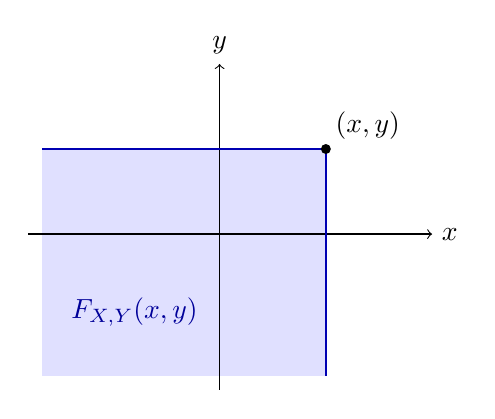
\begin{tikzpicture}[scale=0.9]
\fill[blue!12] (-2.5,-2) rectangle (1.5,1.2);
\draw[->] (-2.7,0) -- (3,0) node[right]{$x$};
\draw[->] (0,-2.2) -- (0,2.4) node[above]{$y$};
\draw[blue!70!black,thick] (1.5,-2) -- (1.5,1.2) -- (-2.5,1.2);
\fill (1.5,1.2) circle (2pt) node[above right]{$(x,y)$};
\node[blue!60!black] at (-1.2,-1.1) {$F_{X,Y}(x,y)$};
\end{tikzpicture}
\end{center}
{\small \lr{CDF} مشترک در نقطه $(x,y)$ برابر جرم احتمال کل ربع صفحه «جنوب‌غربی» این نقطه است.}

\subsection{نحوه استفاده}
از طریق توزیع انباشته مشترک، می‌توان احتمال هر واقعه‌ای در رابطه با دو متغیر تصادفی را محاسبه نمود. برای مثال (\textbf{با استفاده از اصل شمول و عدم شمول!}):
\[
\Prob\big(X>x\ ,\ Y>y\big)=1-F_{XY}(\infty,y)-F_{XY}(x,\infty)+F_{XY}(x,y).
\]
\begin{proof}
متمم رویداد $\{X>x,Y>y\}$ برابر $\{X\le x\}\cup\{Y\le y\}$ است. طبق اصل شمول و عدم شمول:
$\Prob(\{X\le x\}\cup\{Y\le y\})=F_{XY}(x,\infty)+F_{XY}(\infty,y)-F_{XY}(x,y)$. با کم کردن از ۱ حکم ثابت می‌شود.
\end{proof}

\begin{center}
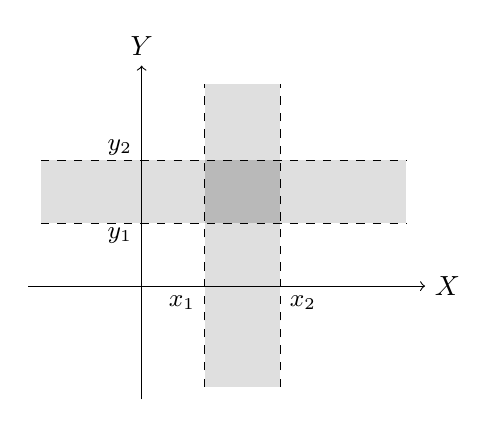
\begin{tikzpicture}[scale=0.8]
\fill[gray!25] (1,-1.6) rectangle (2.2,3.2);
\fill[gray!25] (-1.6,1) rectangle (4.2,2);
\fill[gray!55] (1,1) rectangle (2.2,2);
\draw[->] (-1.8,0) -- (4.5,0) node[right]{$X$};
\draw[->] (0,-1.8) -- (0,3.5) node[above]{$Y$};
\draw[dashed] (1,-1.6) -- (1,3.2); \draw[dashed] (2.2,-1.6) -- (2.2,3.2);
\draw[dashed] (-1.6,1) -- (4.2,1); \draw[dashed] (-1.6,2) -- (4.2,2);
\node[below left,font=\small] at (1,0) {$x_1$}; \node[below right,font=\small] at (2.2,0) {$x_2$};
\node[left,font=\small] at (0,0.8) {$y_1$}; \node[left,font=\small] at (0,2.2) {$y_2$};
\end{tikzpicture}
\end{center}

\begin{question}[$\Prob(x_1\le X\le x_2\ ,\ y_1\le Y\le y_2)=\ ?$ و $\Prob(x_1\le X\le x_2\ \text{\lr{or}}\ y_1\le Y\le y_2)=\ ?$]
\begin{answer}
(برای سادگی فرض کنید متغیرها پیوسته‌اند تا مرزها اهمیتی نداشته باشند.)

\textbf{مستطیل (\lr{and}):} احتمال مستطیل (ناحیه تیره در شکل) با شمول و عدم شمول روی چهار ربع صفحه «جنوب‌غربی» به دست می‌آید:
\[
\boxed{\begin{aligned}\Prob(x_1\le X\le x_2,\ y_1\le Y\le y_2)=\ &F_{XY}(x_2,y_2)-F_{XY}(x_1,y_2)\\&-F_{XY}(x_2,y_1)+F_{XY}(x_1,y_1)\end{aligned}}
\]
(ربع $(x_2,y_2)$ را برمی‌داریم، ربع‌های سمت چپ مستطیل و زیر مستطیل را کم می‌کنیم، و چون ربع $(x_1,y_1)$ دو بار کم شده، یک بار اضافه می‌کنیم.)

\textbf{صلیب (\lr{or}):} اجتماع نوار عمودی و نوار افقی (کل ناحیه سایه‌دار):
\[
\begin{aligned}
\Prob(x_1\le X\le x_2\ \text{\lr{or}}\ y_1\le Y\le y_2)=&\big[F_X(x_2)-F_X(x_1)\big]+\big[F_Y(y_2)-F_Y(y_1)\big]\\
&-\Prob(x_1\le X\le x_2,\ y_1\le Y\le y_2),
\end{aligned}
\]
که در آن $F_X(x)=F_{XY}(x,\infty)$ و $F_Y(y)=F_{XY}(\infty,y)$ و جمله آخر همان احتمال مستطیل بالاست.
\end{answer}
\end{question}

\subsection{توزیع انباشته حاشیه‌ای \lr{(Marginal CDF)}}
پیش‌تر بحث کردیم که \textbf{اطلاعات مشترک} دو متغیر تصادفی در \textbf{توزیع انباشته جداگانه آنان} موجود نیست، و برای دانستن آن نیاز به داشتن تابعی بسیار بزرگ‌تر و غنی‌تر داریم. اما برعکس گزاره فوق صادق است. یعنی، تابع توزیع انباشته جداگانه هر یک از متغیرهای تصادفی از روی توزیع انباشته مشترک قابل حصول است:
\[
\boxed{\ F_X(x)=F_{XY}(x,\infty)\quad,\quad F_Y(y)=F_{XY}(\infty,y)\ }
\]
(زیرا $\{Y\le\infty\}$ همیشه رخ می‌دهد.)

\begin{theorem}[استقلال بر حسب \lr{CDF}]
دو متغیر تصادفی از یکدیگر \textcolor{red!70!black}{مستقل}‌اند اگر و تنها اگر رابطه زیر به ازای تمامی $x,y$ها برقرار باشد:
\[
F_{XY}(x,y)=F_X(x)\times F_Y(y).
\]
\end{theorem}

\section{تابع چگالی احتمال مشترک \lr{(Joint PDF)}}

\begin{definition}[چگالی مشترک]
مطابق پیشین، تابع چگالی احتمال مشترک برای دو متغیر تصادفی $X,Y$ را به صورت زیر تعریف می‌کنیم:
\[
f_{XY}(x,y)=\frac{\partial^2}{\partial x\,\partial y}F_{XY}(x,y).
\]
\end{definition}

\textbf{مفهوم چگالی در حین مشتق‌گیری ظاهر می‌شود:}
\[
f_{XY}(x,y)=\lim_{h,t\to0}\frac{\Prob\big(x\le X\le x+h\ ,\ y\le Y\le y+t\big)}{h\cdot t},
\]
یعنی احتمال یک مستطیل کوچک تقسیم بر \textbf{مساحت} آن (جرم بر واحد سطح). (این از فرمول مستطیل بالا و تعریف مشتق دوم مخلوط به دست می‌آید.)

به عبارت صریح‌تر، احتمال واقعه عام $(X,Y)\in S\subseteq\R^2$ به صورت زیر محاسبه می‌شود:
\[
\Prob(S)=\iint_{(x,y)\in S}f_{XY}(x,y)\dd x\dd y ,
\]
یعنی \textbf{حجم} زیر سطح $f_{XY}$ روی ناحیه $S$.

\section{خواص و حاشیه‌سازی \lr{(Marginalization)}}

\begin{itemize}
\item می‌توان دید که \textbf{تابع چگالی احتمال مشترک} نامنفی بوده و انتگرال آن بر روی تمامی صفحه $\R^2$ برابر با ۱ است.
\item تابع چگالی احتمال حاشیه‌ای برای هر یک از متغیرهای تصادفی به صورت زیر به دست می‌آید:
\[
\boxed{\ f_X(x)=\int_{-\infty}^{\infty}f_{XY}(x,y)\dd y\quad,\quad f_Y(y)=\int_{-\infty}^{\infty}f_{XY}(x,y)\dd x\ }
\]
(این همان قانون احتمال کل در حالت پیوسته است: روی همه مقادیر ممکن متغیر دیگر «جمع» می‌زنیم.)
\item دو متغیر تصادفی $X,Y$ مستقل‌اند، اگر و تنها اگر داشته باشیم:
\[
f_{XY}(x,y)=f_X(x)f_Y(y).
\]
\end{itemize}

\begin{note}
\notetitle \textbf{تصویر هندسی:} چگالی مشترک یک «تپه» روی صفحه $(x_1,x_2)$ با حجم کل ۱ است. چگالی حاشیه‌ای $f_{X_1}$ «سایه» یا تصویر این تپه روی محور $x_1$ است (انتگرال در امتداد $x_2$)؛ مساحت زیر هر حاشیه ۱ است. اگر تپه را با صفحه $x_2=b$ برش دهیم، شکل برش (پس از بهنجارسازی) چگالی شرطی $f_{X_1|X_2}(x_1\given b)$ است (جلسه بعد). در حالت داده‌ها، ابری از نقاط $(x_1,x_2)$ داریم و هیستوگرام هر مؤلفه به‌تنهایی، حاشیه‌ها را تقریب می‌زند.
\end{note}

\begin{center}
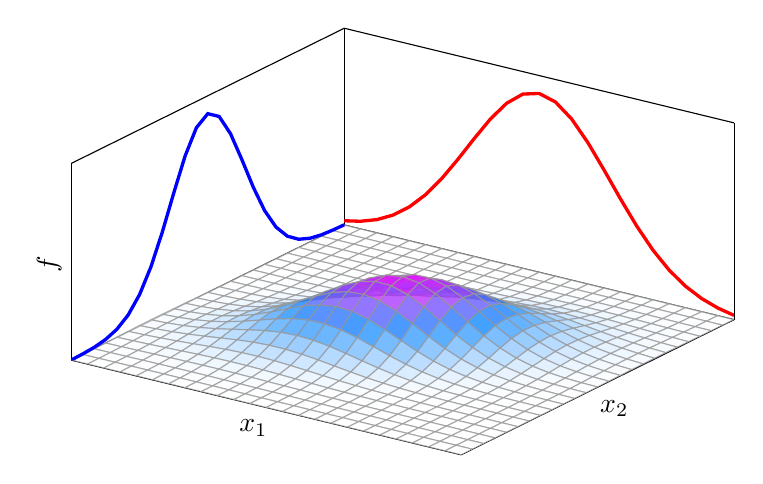
\begin{tikzpicture}
\begin{axis}[view={35}{40},width=10cm,height=7cm,xlabel={$x_1$},ylabel={$x_2$},zlabel={$f$},colormap/cool,samples=25,domain=-3:3,y domain=-3:3,zmin=0,ztick=\empty,xtick=\empty,ytick=\empty]
\addplot3[surf,opacity=0.75,faceted color=black!40] {exp(-(x^2 - 1.2*x*y + 1.5*y^2)/1.6)/(2*pi)};
\addplot3[red,very thick,samples y=0,domain=-3:3] (x,3,{0.45*exp(-x^2/2.4)});
\addplot3[blue,very thick,samples y=0,domain=-3:3] (-3,x,{0.45*exp(-x^2/1.3)});
\end{axis}
\end{tikzpicture}\\
{\small یک چگالی مشترک دو متغیره (سطح) و حاشیه‌های آن (منحنی‌های قرمز و آبی روی دیواره‌ها، به صورت نمادین)}
\end{center}

\begin{example}[چگالی مشترک روی مربع واحد]
فرض کنید $f_{XY}(x,y)=x+y$ برای $0\le x,y\le1$ و صفر در غیر این صورت.
(الف) نشان دهید این یک چگالی معتبر است. (ب) چگالی‌های حاشیه‌ای را بیابید. (ج) آیا $X$ و $Y$ مستقل‌اند؟ (د) $\Prob(X+Y\le1)$ را حساب کنید.
\begin{solution}
(الف) نامنفی است و $\int_0^1\!\int_0^1(x+y)\dd x\dd y=\frac12+\frac12=1$.

(ب) $f_X(x)=\int_0^1(x+y)\dd y=x+\frac12$ برای $0\le x\le1$؛ به طور متقارن $f_Y(y)=y+\frac12$.

(ج) $f_X(x)f_Y(y)=(x+\frac12)(y+\frac12)=xy+\frac{x+y}{2}+\frac14\neq x+y$ (مثلاً در $(0,0)$: $\frac14\neq0$). پس مستقل نیستند.

(د) ناحیه مثلث $\{x,y\ge0,\ x+y\le1\}$ است:
\[
\int_0^1\!\!\int_0^{1-x}(x+y)\dd y\dd x=\int_0^1\Big[x(1-x)+\frac{(1-x)^2}{2}\Big]\dd x=\int_0^1\frac{1-x^2}{2}\dd x=\frac12\Big(1-\frac13\Big)=\frac13 .
\]
\end{solution}
\end{example}

\begin{example}[چگالی یکنواخت روی مثلث]
$(X,Y)$ به‌طور یکنواخت روی مثلث $0\le y\le x\le1$ توزیع شده است. چگالی مشترک و حاشیه‌ها را بیابید.
\begin{solution}
مساحت مثلث $\frac12$ است؛ پس $f_{XY}=2$ روی مثلث. حاشیه‌ها:
$f_X(x)=\int_0^x2\dd y=2x$ ($0\le x\le1$) و $f_Y(y)=\int_y^12\dd x=2(1-y)$ ($0\le y\le1$).
مستقل نیستند: حاصل‌ضرب $4x(1-y)$ روی کل مربع مثبت است، اما چگالی مشترک در ناحیه $y>x$ صفر است. \textbf{قاعده سرانگشتی:} اگر تکیه‌گاه چگالی مشترک «مستطیلی» (ضرب دکارتی) نباشد، متغیرها حتماً وابسته‌اند.
\end{solution}
\end{example}

\begin{center}
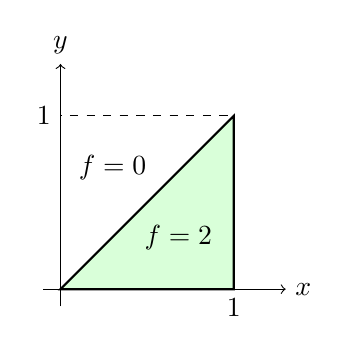
\begin{tikzpicture}[scale=2.2]
\fill[green!15] (0,0) -- (1,0) -- (1,1) -- cycle;
\draw[->] (-0.1,0) -- (1.3,0) node[right]{$x$};
\draw[->] (0,-0.1) -- (0,1.3) node[above]{$y$};
\draw[thick] (0,0) -- (1,0) -- (1,1) -- cycle;
\draw[dashed] (0,0) -- (0,1) -- (1,1);
\node at (0.68,0.3) {$f=2$};
\node at (0.3,0.7) {$f=0$};
\node[below] at (1,0) {$1$}; \node[left] at (0,1) {$1$};
\end{tikzpicture}
\end{center}

\begin{example}[دو نمایی مستقل]
$X,Y$ مستقل و هر دو $\mathrm{Exp}(1)$ هستند. $\Prob(X<Y)$ و $\Prob(X+Y\le1)$ را حساب کنید.
\begin{solution}
$f_{XY}(x,y)=e^{-x}e^{-y}$ برای $x,y\ge0$.
\[
\Prob(X<Y)=\int_0^\infty\!\!\int_x^\infty e^{-x}e^{-y}\dd y\dd x=\int_0^\infty e^{-2x}\dd x=\frac12
\]
(که از تقارن نیز واضح است).
\[
\begin{aligned}
\Prob(X+Y\le1)&=\int_0^1\!\!\int_0^{1-x}e^{-x-y}\dd y\dd x=\int_0^1e^{-x}\big(1-e^{-(1-x)}\big)\dd x\\
&=(1-e^{-1})-e^{-1}=1-\frac2e\approx0.264 .
\end{aligned}
\]
\end{solution}
\end{example}

\section{توزیع مشترک چند متغیر تصادفی}

\subsection{تعریف ریاضیاتی}
\begin{definition}
متغیرهای تصادفی $X_1,X_2,\ldots,X_n$ دارای تابع توزیع انباشته مشترک به صورت زیر خواهند بود:
\[
F_{X_1,\ldots,X_n}(x_1,\ldots,x_n)=\Prob\big(X_1\le x_1,\ldots,X_n\le x_n\big).
\]
متغیرهای تصادفی فوق را (به طور متقابل) مستقل می‌نامیم، اگر و تنها اگر:
\[
F_{X_1,\ldots,X_n}(x_1,\ldots,x_n)=\prod_{i=1}^{n}F_{X_i}(x_i).
\]
\end{definition}
\begin{note}
\notetitle در اسلاید از عبارت «دو به دو مستقل» استفاده شده است؛ اما دقت کنید که شرط ضربی بالا برای \emph{همه} $n$ متغیر با هم، در واقع \textbf{استقلال متقابل} را تعریف می‌کند که از استقلال دوبه‌دو قوی‌تر است (مثال جلسه سوم را به یاد آورید). با قرار دادن $x_j=\infty$ برای برخی اندیس‌ها، از این شرط استقلال هر زیرمجموعه (از جمله هر دو تا) نتیجه می‌شود.
\end{note}

\subsection{تابع چگالی احتمال مشترک: تعریف و حاشیه‌سازی}
برای متغیرهای تصادفی $X_1,X_2,\ldots,X_n$ تابع چگالی احتمال مشترک به صورت زیر تعریف می‌شود:
\[
f_{X_1,\ldots,X_n}(x_1,\ldots,x_n)=\frac{\partial^n}{\partial x_1\cdots\partial x_n}F_{X_1,\ldots,X_n}(x_1,\ldots,x_n).
\]
برای متغیرهای تصادفی منتخب $X_{\eta_1},\ldots,X_{\eta_m}\subset\{X_1,\ldots,X_n\}$ داریم:
\[
f_{X_{\eta_1},\ldots,X_{\eta_m}}=\int_\R\cdots\int_\R f_{X_1,\ldots,X_n}(x_1,\ldots,x_n)\prod_{i\notin\{\eta_1,\ldots,\eta_m\}}\dd x_i ,
\]
یعنی بر روی تمامی اندیس‌هایی که در بین $\eta_1,\ldots,\eta_m$ نیستند باید انتگرال گرفت.

\begin{example}[حاشیه‌سازی سه متغیره]
$f(x,y,z)=6$ روی ناحیه $0\le x\le y\le z\le1$ (و صفر در جای دیگر). چگالی حاشیه‌ای $(X,Z)$ و چگالی $Z$ را بیابید.
\begin{solution}
حجم ناحیه $\frac16$ است (یکی از $3!$ ترتیب ممکن)، پس چگالی ثابت ۶ درست است.
$f_{XZ}(x,z)=\int_x^z6\dd y=6(z-x)$ برای $0\le x\le z\le1$.
$f_Z(z)=\int_0^z6(z-x)\dd x=3z^2$ برای $0\le z\le1$. (بررسی: $\int_0^13z^2=1$.) جالب است که این همان توزیع ماکزیمم سه یکنواخت مستقل است ــ و در واقع $(X,Y,Z)$ در اینجا همان «آماره‌های مرتب» سه یکنواخت مستقل است.
\end{solution}
\end{example}

\section{تمرین‌های تکمیلی}

\begin{exercise}
$F_{XY}(x,y)=(1-e^{-x})(1-e^{-2y})$ برای $x,y\ge0$. آیا $X,Y$ مستقل‌اند؟ $f_{XY}$ و $\Prob(X>1,Y>1)$ را بیابید.
\end{exercise}
\begin{solution}
\lr{CDF} به صورت حاصل‌ضرب $F_X(x)F_Y(y)$ با $F_X=1-e^{-x}$ و $F_Y=1-e^{-2y}$ است؛ پس مستقل‌اند ($X\sim\mathrm{Exp}(1)$ و $Y\sim\mathrm{Exp}(2)$). $f_{XY}=\frac{\partial^2F}{\partial x\partial y}=e^{-x}\cdot2e^{-2y}$.
$\Prob(X>1,Y>1)=1-F(\infty,1)-F(1,\infty)+F(1,1)=e^{-1}e^{-2}=e^{-3}\approx0.0498$.
\end{solution}

\begin{exercise}
نقطه‌ای به‌طور یکنواخت درون دایره واحد انتخاب می‌شود. چگالی حاشیه‌ای مختص $X$ را بیابید. آیا $X$ و $Y$ مستقل‌اند؟
\end{exercise}
\begin{solution}
$f_{XY}=\frac1\pi$ داخل دایره. $f_X(x)=\int_{-\sqrt{1-x^2}}^{\sqrt{1-x^2}}\frac1\pi\dd y=\frac{2}{\pi}\sqrt{1-x^2}$ برای $|x|\le1$ (نیم‌دایره). مستقل نیستند: تکیه‌گاه مستطیلی نیست؛ مثلاً $f_{XY}(0.9,0.9)=0$ ولی $f_X(0.9)f_Y(0.9)>0$.
\end{solution}

\begin{exercise}
برای متغیرهای گسسته، \lr{PMF} مشترک $P(x,y)=c(x+y)$ با $x,y\in\{1,2\}$ است. $c$، حاشیه‌ها و $\Prob(X=Y)$ را بیابید.
\end{exercise}
\begin{solution}
$\sum=c(2+3+3+4)=12c=1\Rightarrow c=\frac1{12}$. $P_X(1)=\frac{2+3}{12}=\frac5{12}$ و $P_X(2)=\frac7{12}$ (برای $Y$ نیز همین). $\Prob(X=Y)=\frac{2+4}{12}=\frac12$. مستقل نیستند: $P(1,1)=\frac2{12}\ne\frac{25}{144}$.
\end{solution}
